%Part of/Parte di https://github.com/f-dinucci/appuntiMeccanicaFluidi/
%License/Licenza Creative Commons Attribution-ShareAlike 4.0 International (CC BY-SA 4.0) - attribution/attribuzione Francesco Di Nucci
%See also/Vedere anche https://creativecommons.org/licenses/by-sa/4.0/ and/e https://creativecommons.org/licenses/by-sa/4.0/legalcode
%
\section{Correnti ad alto numero di Reynolds}
\subsection{Approssimazioni per alto numero di Reynolds}
Si vedrà ora cosa accade nel caso di numero di Reynolds grande.
Si parte dalle equazioni in forma adimensionale, considerando solamente la pressione dinamica, si vede che è come se le equazioni di Eulero fossero un'approssimazione delle equazioni di Navier-Stokes per Reynolds grande.
Cambiano inoltre le condizioni al contorno su una parete solida:
%
	\begin{equation*}
		\begin{gathered}
			\div{\uline{v}} = 0 \rightarrow \uline{n} \vdot \uline{v} = 0\\
			\pdv{\uline{v}}{t} + \uline{v} \vdot \grad{\uline{v}} + \grad{p} = \cancel{\frac{1}{R_e} \nabla_2 \uline{v}}
		\end{gathered}
	\end{equation*}
%
Le equazioni di Eulero e Navier-Stokes alla parete presentano quindi comportamenti diversi
 %
	\begin{figure}[ht]
		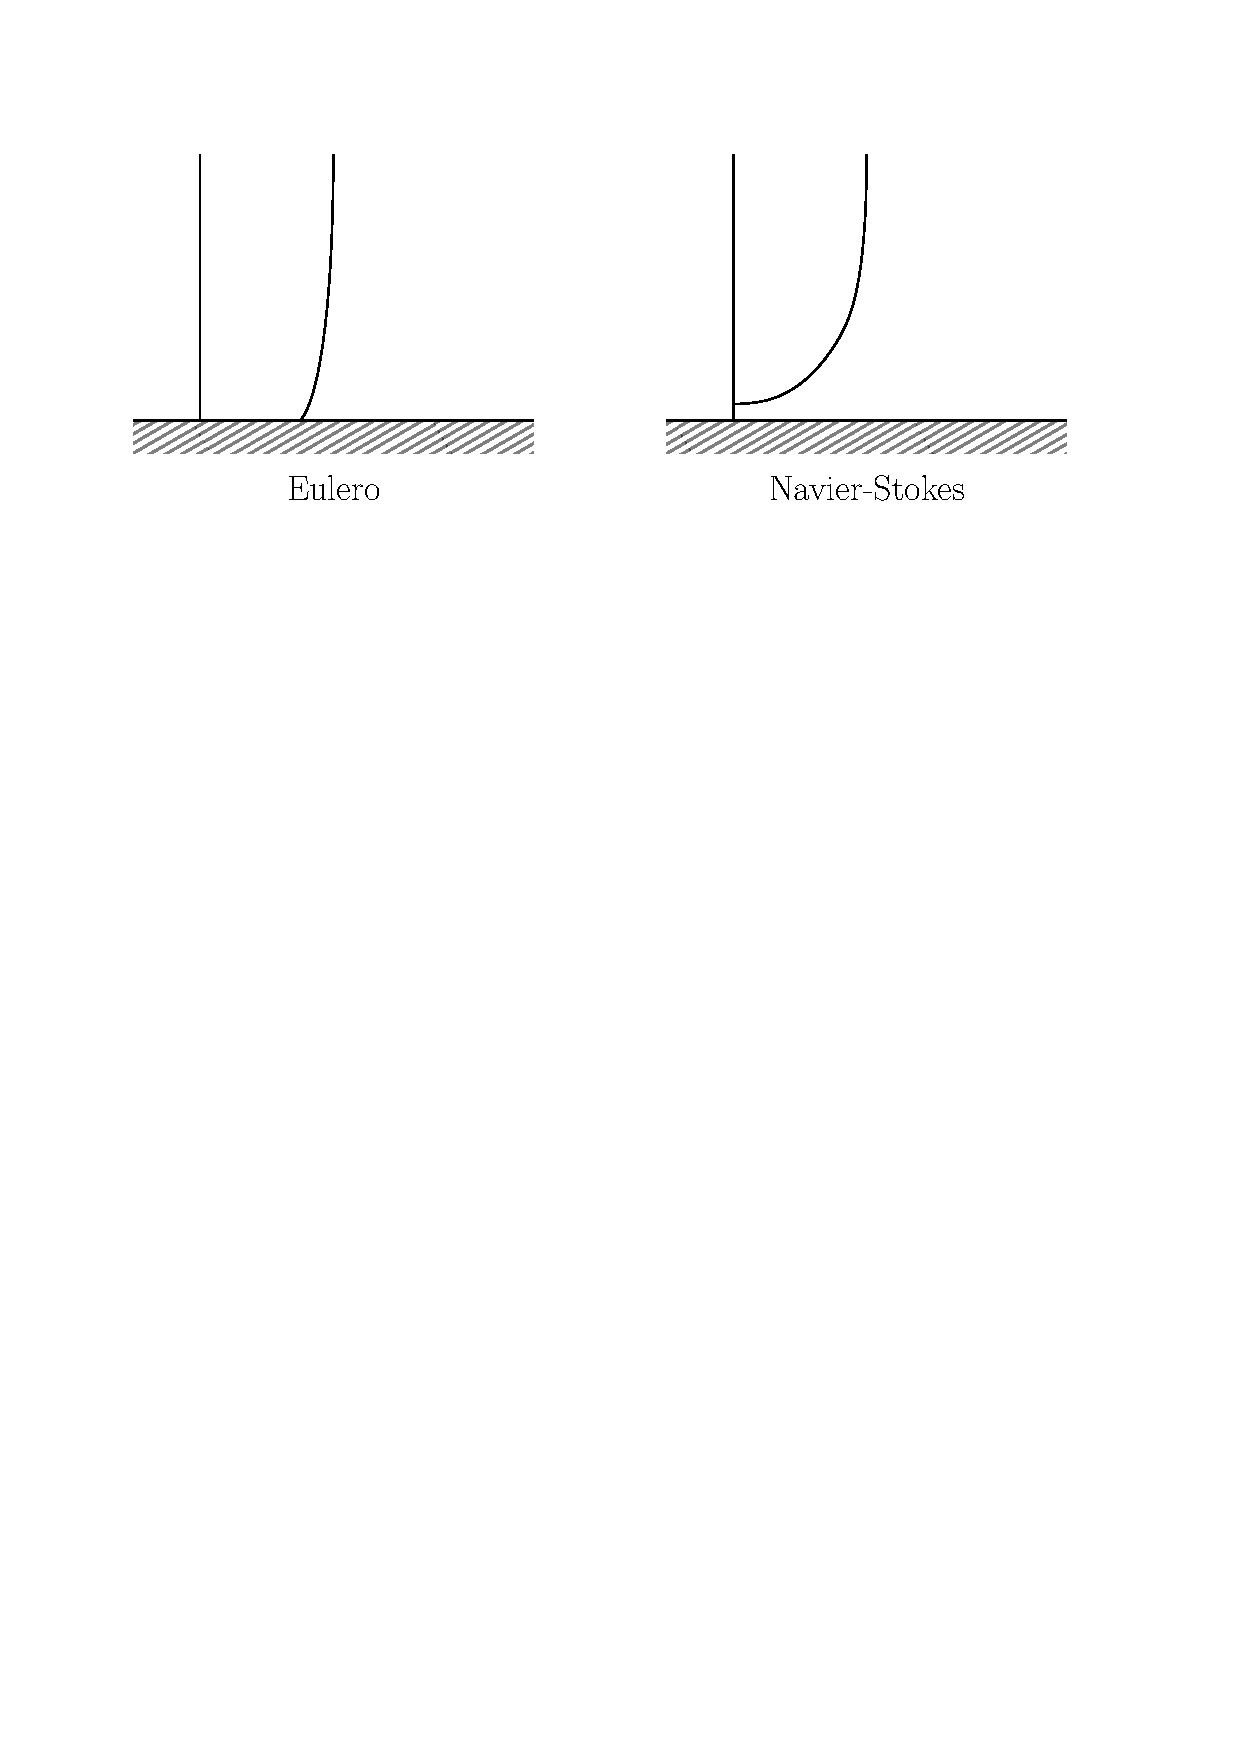
\includegraphics[scale=0.7]{./7.1 Correnti ad alto numero di Reynolds/7.1-1}
		\centering
		\caption{Comportamento alla parete}
	\end{figure}
%
Per Reynolds tendente ad infinito questi devono tendere uno all'altro in una zona detta di strato limite, si vedrà poi che le equazioni di Eulero valgono solamente fino ad una certa distanza dalla parete e che lo strato limite va analizzato diversamente.

Si ricordano prima vorticità ed equazione in forma di Crocco:
%
	\begin{equation*}
		\begin{gathered}
			\uline{\omega} = \curl{\uline{v}}\\
			\pdv{\uline{v} }{t} + \uline{\omega} \cross \uline{v} + \grad{\left( p + \frac{v^2}{2} \right)} = 0
		\end{gathered}
	\end{equation*}
%
Prendendo il rotore di tutta l'equazione si ricava l'equazione di trasporto della vorticità:
%
	\begin{equation*}
		\pdv{\uline{\omega}}{t} + \curl{\left( \uline{\omega} \cross \uline{v} \right)} = 0
	\end{equation*}
%
È una equazione non lineare, $\omega$ e $v$ sono sempre legate.
Se la vorticità è nulla, sono nulli ambedue i termini.
Una possibile soluzione è $\uline{\omega} = 0$, che è un moto irrotazionale, si vede quindi che il caso di vorticità nulla, ipotizzato per le equazioni di Bernoulli in forma forte, può effettivamente capitare.
Notare che esistono anche soluzioni in caso di vorticità non nulla.

In questo caso il problema è lineare (la somma di due soluzioni è a sua volta una soluzione, si possono cercare soluzioni per sovrapposizione degli effetti) e diventa:
%
	\begin{equation*}
		\begin{gathered}
			\curl{\uline{v}} = 0\\
			\div{\uline{v}} = 0
			\end{gathered}
	\end{equation*}
%
Dato che il rotore è nullo, si può trovare gradiente del potenziale e calcolarne la divergenza, il moto irrotazionale si riduce ad una sola equazione:
%
	\begin{equation*}
		\begin{gathered}
			\uline{v} = \grad{\phi}\\
			\div{\grad{\phi}} = \laplacian{\phi} = 0
		\end{gathered}
	\end{equation*}
%

\subsection*{Bibliografia 7.1}
\cite[Cap.\ 10.4]{CengelCimbala}\\
\cite[Cap.\ 10.1, 10.2]{PnueliGutfinger}